

\documentclass[bigger]{beamer}

\usepackage{style}
\usepackage{subfiles}


\title[STG vs GRIN] %optional
{Comparing STG and GRIN}

\author[P. Podlovics, Cs. Hruska, Andor Pénzes ] % (optional, for multiple authors)
{Péter Podlovics, Csaba Hruska, Andor Pénzes}

\institute[ELTE] % (optional)
{
	Eötvös Loránd University (ELTE), \\ Budapest, Hungary
}

\date{Haskell meetup} % (optional)



\begin{document}

{
	\usebackgroundtemplate{
\includegraphics[width=\paperwidth]{title.jpg}}%
	\frame{\vspace{15mm}\titlepage}
}

\begin{frame}
	\frametitle{Overview}
	\tableofcontents
\end{frame}

\section{Codes}

\begin{frame}[fragile]
\frametitle{Why functional?}

\begin{vfitemize}
	\item Declarativeness
	\begin{itemize}
		\item[pro:] can program on a higher abstraction level
	\end{itemize}
	\item Composability\\
	\begin{itemize}
		\item[pro:] can easily piece together smaller programs
		\item[con:] results in a lot of function calls
	\end{itemize}
	\item Functions are first class citizens
	\begin{itemize}
		\item[pro:] higher order functions
		\item[con:] unknown function calls
	\end{itemize}
\end{vfitemize}

\end{frame}

\begin{frame}[fragile]
\frametitle{High level overview}

\begin{minipage}{0.4\textwidth}
	\begin{center}
		Spineless Tagless G-machine
	\end{center}
	\begin{itemize}
		\item<2-> higher order functional language
		\item<3-> execution of lambda calculus
		\item<4-> implicit operational semantics
		% op.sem. is detached from the language
		% can't really guess how the program is executed just by looking at the code
		\item<5-> efficient code generation
	\end{itemize}
\end{minipage}
\hfill
\begin{minipage}{0.4\textwidth}
	\begin{center}
		Graph Reduction Intermediate Notation
	\end{center}
	\begin{itemize}
		\item<6-> first order imperative language
		\item<7-> unified back end for functional languages
		\item<8-> explicit operational semantics
		% op.sem. closely tied together with the language
		% all functional constructs can be expressed using really simple and transparent language constructs (transparent as in we see what is happening)
		\item<9-> aggressive code optimization 
	\end{itemize}
\end{minipage}

\end{frame}

%%%%%%%% STG Overview %%%%%%%%%%

\begin{frame}[fragile]
\frametitle{STG overview}
\begin{center}

	\begin{minipage}{0.25\textwidth}
		\begin{figure}
			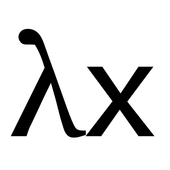
\includegraphics[scale=0.4]{lambda-icon.png}
		\end{figure}
	\end{minipage}
	\hfill
	\pause
	\begin{minipage}{0.30\textwidth}
		\begin{figure}
			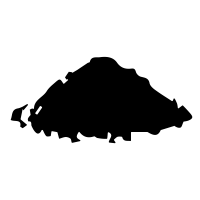
\includegraphics[scale=0.3]{heap-icon.png}
		\end{figure}
	\end{minipage}
	\hfill
	\pause
	\begin{minipage}{0.30\textwidth}
		\begin{figure}
			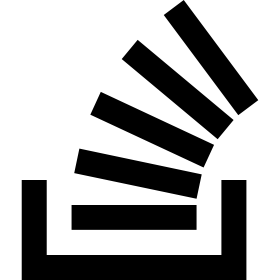
\includegraphics[scale=0.04]{stack-icon.png}
		\end{figure}
	\end{minipage}

\end{center}
\end{frame}

\begin{frame}[fragile]
\frametitle{STG overview}
\begin{center}

	\begin{minipage}{0.30\textwidth}
		\vspace{1cm}
		\begin{figure}
			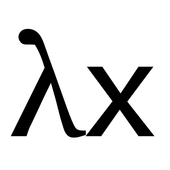
\includegraphics[scale=0.45]{lambda-icon.png}
		\end{figure}
		\onslide<2>
		\begin{haskellcode}
			and :: Bool -> Bool -> Bool
		\end{haskellcode}
		\vspace{-0.4cm}
		\onslide<2-3>
		\begin{haskellcode}
			and True True = True
			and _    _    = False
		\end{haskellcode}
	\end{minipage}
	\hfill
	\onslide<1-3>
	\begin{minipage}{0.30\textwidth}
		\begin{figure}
			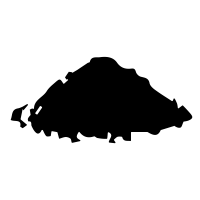
\includegraphics[scale=0.3]{heap-icon.png}
		\end{figure}
	\end{minipage}
	\hfill
	\begin{minipage}{0.30\textwidth}
		\begin{figure}
			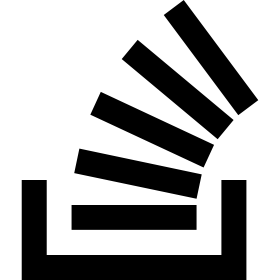
\includegraphics[scale=0.04]{stack-icon.png}
		\end{figure}
	\end{minipage}

\end{center}
\end{frame}

\begin{frame}[fragile]
\frametitle{STG overview}
\begin{center}

	\begin{minipage}{0.30\textwidth}
		\vspace{1.8cm}
		\begin{figure}
			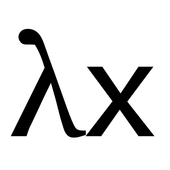
\includegraphics[scale=0.45]{lambda-icon.png}
		\end{figure}
		\begin{haskellcode}
			and x y = case x of
			  True -> case y of
			    True -> True
			    y' -> False
			  x' -> False
		\end{haskellcode}
	\end{minipage}
	\hfill
	\begin{minipage}{0.30\textwidth}
		\begin{figure}
			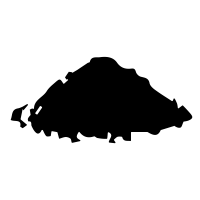
\includegraphics[scale=0.3]{heap-icon.png}
		\end{figure}
	\end{minipage}
	\hfill
	\begin{minipage}{0.30\textwidth}
		\begin{figure}
			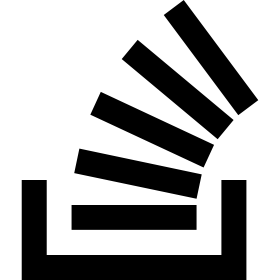
\includegraphics[scale=0.04]{stack-icon.png}
		\end{figure}
	\end{minipage}

\end{center}
\end{frame}

\begin{frame}[fragile]
\frametitle{STG overview}
\begin{center}

	\begin{minipage}{0.30\textwidth}
		\vspace{1.8cm}
		\begin{figure}
			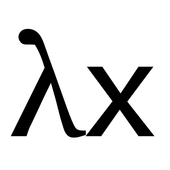
\includegraphics[scale=0.45]{lambda-icon.png}
		\end{figure}
		\begin{haskellcode}
			and = \x y -> case x of
			  True -> case y of
			    True -> True
			    y' -> False
			  x' -> False
		\end{haskellcode}
	\end{minipage}
	\hfill
	\begin{minipage}{0.30\textwidth}
		\begin{figure}
			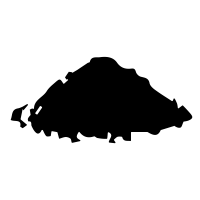
\includegraphics[scale=0.3]{heap-icon.png}
		\end{figure}
	\end{minipage}
	\hfill
	\begin{minipage}{0.30\textwidth}
		\begin{figure}
			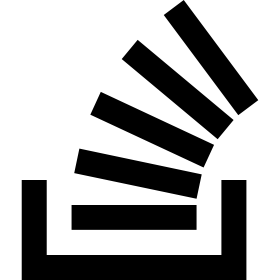
\includegraphics[scale=0.04]{stack-icon.png}
		\end{figure}
	\end{minipage}

\end{center}
\end{frame}

\begin{frame}[fragile]
\frametitle{STG overview}
\begin{center}

	\begin{minipage}{0.25\textwidth}
		\begin{figure}
			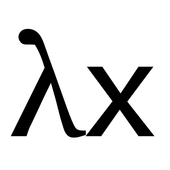
\includegraphics[scale=0.4]{lambda-icon.png}
		\end{figure}
	\end{minipage}
	\hfill
	\begin{minipage}{0.30\textwidth}
		\begin{figure}
			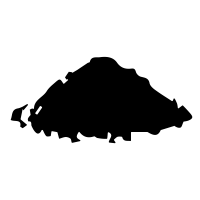
\includegraphics[scale=0.35]{heap-icon.png}
		\end{figure}
	\end{minipage}
	\hfill
	\begin{minipage}{0.30\textwidth}
		\begin{figure}
			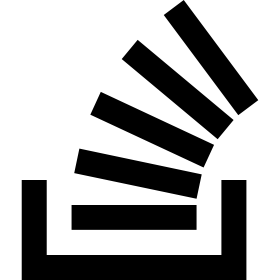
\includegraphics[scale=0.04]{stack-icon.png}
		\end{figure}
	\end{minipage}

\end{center}
\end{frame}

\begin{frame}[fragile]
\frametitle{STG overview}
\begin{center}

	\begin{minipage}{0.15\textwidth}
		\begin{figure}
			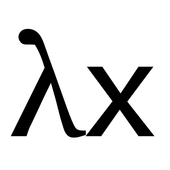
\includegraphics[scale=0.4]{lambda-icon.png}
		\end{figure}
	\end{minipage}
	\hfill
	\begin{minipage}{0.30\textwidth}
		\vspace{1cm}
		\begin{figure}
			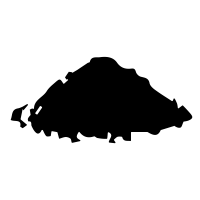
\includegraphics[scale=0.35]{heap-icon.png}
		\end{figure}
		\vspace{-1cm}
		\begin{figure}
			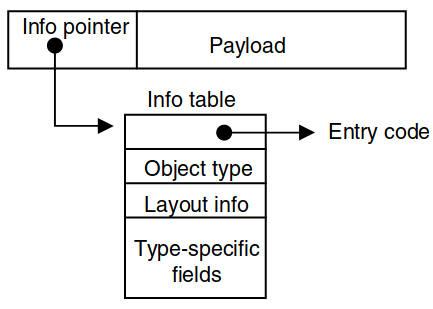
\includegraphics[scale=0.33]{heap-object.png}
		\end{figure}
	\end{minipage}
	\hfill
	\begin{minipage}{0.30\textwidth}
		\begin{figure}
			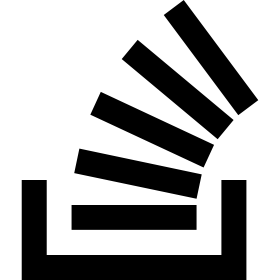
\includegraphics[scale=0.04]{stack-icon.png}
		\end{figure}
	\end{minipage}

\end{center}
\end{frame}

\begin{frame}[fragile]
\frametitle{STG overview}
\begin{center}

	\begin{minipage}{0.25\textwidth}
		\begin{figure}
			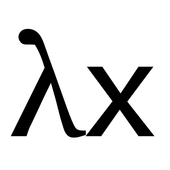
\includegraphics[scale=0.4]{lambda-icon.png}
		\end{figure}
	\end{minipage}
	\hfill
	\begin{minipage}{0.30\textwidth}
		\begin{figure}
			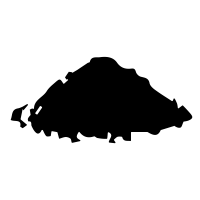
\includegraphics[scale=0.3]{heap-icon.png}
		\end{figure}
	\end{minipage}
	\hfill
	\begin{minipage}{0.30\textwidth}
		\begin{figure}
			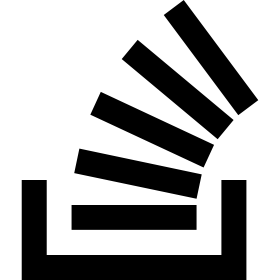
\includegraphics[scale=0.04]{stack-icon.png}
		\end{figure}
	\end{minipage}

\end{center}
\end{frame}

\begin{frame}[fragile]
\frametitle{STG overview}
\begin{center}

	\begin{minipage}{0.25\textwidth}
		\begin{figure}
			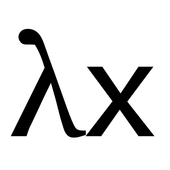
\includegraphics[scale=0.4]{lambda-icon.png}
		\end{figure}
	\end{minipage}
	\hfill
	\begin{minipage}{0.30\textwidth}
		\begin{figure}
			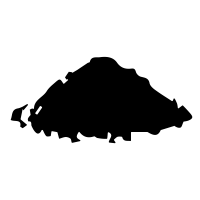
\includegraphics[scale=0.3]{heap-icon.png}
		\end{figure}
	\end{minipage}
	\hfill
	\begin{minipage}{0.30\textwidth}
		\vspace{1cm}
		\begin{figure}
			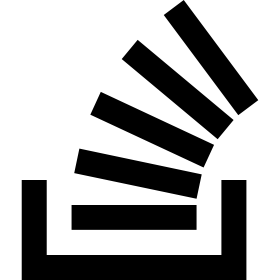
\includegraphics[scale=0.05]{stack-icon.png}
		\end{figure}
		\begin{haskellcode}
			case * of {...}
		\end{haskellcode}
		\pause
		\begin{haskellcode}
			Update x *
		\end{haskellcode}
		\pause
		\begin{haskellcode}
			* x y z
		\end{haskellcode}
	\end{minipage}

\end{center}
\end{frame}

\begin{frame}[fragile]
\frametitle{STG overview}
\begin{center}

	\begin{minipage}{0.25\textwidth}
		\begin{figure}
			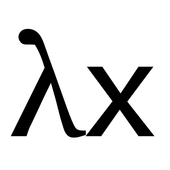
\includegraphics[scale=0.4]{lambda-icon.png}
		\end{figure}
	\end{minipage}
	\hfill
	\begin{minipage}{0.30\textwidth}
		\begin{figure}
			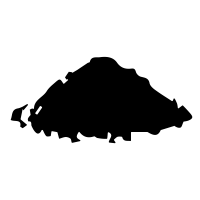
\includegraphics[scale=0.3]{heap-icon.png}
		\end{figure}
	\end{minipage}
	\hfill
	\begin{minipage}{0.30\textwidth}
		\begin{figure}
			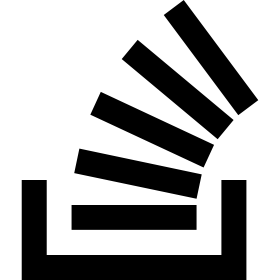
\includegraphics[scale=0.04]{stack-icon.png}
		\end{figure}
	\end{minipage}

\end{center}
\end{frame}

\begin{frame}[fragile]
\frametitle{STG overview}
\begin{center}

	\begin{minipage}{0.30\textwidth}
		\vspace{-3cm}
		\begin{haskellcode}
			and = \x y -> case x of
			 True -> case y of
			  True -> True
			   y' -> False
			 x' -> False
		\end{haskellcode}
	\end{minipage}
	\hfill
	\begin{minipage}{0.30\textwidth}
		\vspace{0.75cm}
		\begin{figure}
			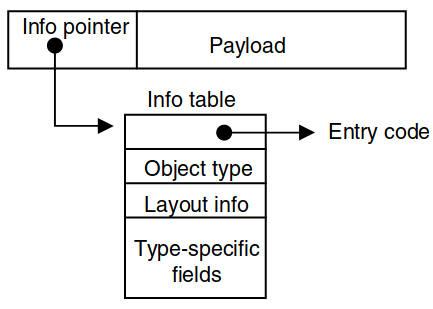
\includegraphics[scale=0.30]{heap-object.png}
		\end{figure}
	\end{minipage}
	\hfill
	\begin{minipage}{0.30\textwidth}
		\vspace{5cm}
		\begin{haskellcode}
			case * of {...}
			Update x *
			* x y z
		\end{haskellcode}
	\end{minipage}

\end{center}
\end{frame}

%%%%%%%%%% STG Examples %%%%%%%%%%%

\begin{frame}[fragile]
\frametitle{STG id-add}
\begin{center}

	\begin{haskellcode}
		id = \x -> x
	\end{haskellcode}
	\pause
	\begin{haskellcode}
		zero = \ -> Int# 0#;
		one  = \ -> Int# 1#;
	\end{haskellcode}
	\pause
	\begin{haskellcode}
		add = \x y -> case x of
		  Int# x' -> case y of
		    Int# y' -> case +# x' y' of
		      r -> Int# r;
		    badInt -> Error_min badInt;
		  badInt -> Error_min badInt;
	\end{haskellcode}
	\pause
	\begin{haskellcode}
		main = \ -> let add_one = \ -> add one
		            in id add_one zero
	\end{haskellcode}

\end{center}
\end{frame}


\begin{frame}[fragile]
\frametitle{STG id-add}
\begin{center}

	\begin{haskellcode}
		id = \x -> x
	\end{haskellcode}
	\begin{haskellcode}
		zero = \ -> Int# 0#;
		one  = \ -> Int# 1#;
	\end{haskellcode}
	\begin{haskellcode}
		add = \x y -> case x of
		  Int# x' -> case y of
		    Int# y' -> case +# x' y' of
		      r -> Int# r;
		    badInt -> Error_min badInt;
		  badInt -> Error_min badInt;
	\end{haskellcode}
	\begin{haskellcode}
		main = \ => let add_one = \ -> add one
		            in id add_one zero
	\end{haskellcode}

\end{center}
\end{frame}



%%%%%% GRIN Overview %%%%%%%%%

\begin{frame}[fragile]
\frametitle{GRIN overview}
\begin{center}

	\begin{minipage}{0.30\textwidth}
		\begin{figure}
			
\includegraphics[scale=0.20]{algebra.png}
		\end{figure}
	\end{minipage}
	\hfill
	\pause
	\begin{minipage}{0.30\textwidth}
		\begin{figure}
			
\includegraphics[scale=0.15]{graph-reduction.png}
		\end{figure}
	\end{minipage}
	\hfill
	\pause
	\begin{minipage}{0.30\textwidth}
		\begin{figure}
			
\includegraphics[scale=0.15]{whole-program-compilation.png}
		\end{figure}
	\end{minipage}

\end{center}
\end{frame}

\begin{frame}[fragile]
\frametitle{GRIN overview}
\begin{center}

	\begin{minipage}{0.30\textwidth}
		\begin{figure}
			
\includegraphics[scale=0.25]{algebra.png}
		\end{figure}
	\end{minipage}
	\hfill
	\begin{minipage}{0.30\textwidth}
		\begin{figure}
			
\includegraphics[scale=0.15]{graph-reduction.png}
		\end{figure}
	\end{minipage}
	\hfill
	\begin{minipage}{0.30\textwidth}
		\begin{figure}
			
\includegraphics[scale=0.15]{whole-program-compilation.png}
		\end{figure}
	\end{minipage}

\end{center}
\end{frame}

\begin{frame}[fragile]
\frametitle{GRIN overview}
\begin{center}

	\begin{minipage}{0.30\textwidth}
		\vspace{1cm}
		\begin{figure}
			
\includegraphics[scale=0.25]{algebra.png}
		\end{figure}
		\vspace{-0.5cm}
		\begin{itemize}
			\item<1-> C-node
			\item<2-> F-node
			\item<3-> P-node
		\end{itemize}
	\end{minipage}
	\hfill
	\begin{minipage}{0.30\textwidth}
		\begin{figure}
			
\includegraphics[scale=0.15]{graph-reduction.png}
		\end{figure}
	\end{minipage}
	\hfill
	\begin{minipage}{0.30\textwidth}
		\begin{figure}
			
\includegraphics[scale=0.15]{whole-program-compilation.png}
		\end{figure}
	\end{minipage}

\end{center}
\end{frame}


\begin{frame}[fragile]
\frametitle{GRIN overview}
\begin{center}

	\begin{minipage}{0.30\textwidth}
		\begin{figure}
			
\includegraphics[scale=0.20]{algebra.png}
		\end{figure}
	\end{minipage}
	\hfill
	\begin{minipage}{0.30\textwidth}
		\begin{figure}
			
\includegraphics[scale=0.20]{graph-reduction.png}
		\end{figure}
	\end{minipage}
	\hfill
	\begin{minipage}{0.30\textwidth}
		\begin{figure}
			
\includegraphics[scale=0.15]{whole-program-compilation.png}
		\end{figure}
	\end{minipage}

\end{center}
\end{frame}

\begin{frame}[fragile]
\frametitle{GRIN overview}
\begin{center}

	\begin{minipage}{0.30\textwidth}
		\begin{figure}
			
\includegraphics[scale=0.20]{algebra.png}
		\end{figure}
	\end{minipage}
	\hfill
	\begin{minipage}{0.30\textwidth}
		\vspace{1cm}
		\begin{figure}
			
\includegraphics[scale=0.20]{graph-reduction.png}
		\end{figure}
		\vspace{-0.5cm}
		\begin{itemize}
			\item<1-> store
			\item<2-> fetch
			\item<3-> update
		\end{itemize}
	\end{minipage}
	\hfill
	\begin{minipage}{0.30\textwidth}
		\begin{figure}
			
\includegraphics[scale=0.15]{whole-program-compilation.png}
		\end{figure}
	\end{minipage}

\end{center}
\end{frame}

\begin{frame}[fragile]
\frametitle{GRIN overview}
\begin{center}

	\begin{minipage}{0.30\textwidth}
		\begin{figure}
			
\includegraphics[scale=0.20]{algebra.png}
		\end{figure}
	\end{minipage}
	\hfill
	\begin{minipage}{0.30\textwidth}
		\begin{figure}
			
\includegraphics[scale=0.15]{graph-reduction.png}
		\end{figure}
	\end{minipage}
	\hfill
	\begin{minipage}{0.30\textwidth}
		\begin{figure}
			
\includegraphics[scale=0.20]{whole-program-compilation.png}
		\end{figure}
	\end{minipage}

\end{center}
\end{frame}

\begin{frame}[fragile]
\frametitle{GRIN overview}
\begin{center}

	\begin{minipage}{0.30\textwidth}
		\begin{figure}
			
\includegraphics[scale=0.20]{algebra.png}
		\end{figure}
	\end{minipage}
	\hfill
	\begin{minipage}{0.30\textwidth}
		\begin{figure}
			
\includegraphics[scale=0.15]{graph-reduction.png}
		\end{figure}
	\end{minipage}
	\hfill
	\begin{minipage}{0.30\textwidth}
		\vspace{1cm}
		\begin{figure}
			\includegraphics[scale=0.20]{whole-program-compilation.png}
		\end{figure}
		\vspace{-0.5cm}
		\begin{itemize}
			\item<1-> eval
			\item<2-> apply
			\item<3-> analyses
		\end{itemize}
	\end{minipage}

\end{center}
\end{frame}

\begin{frame}[fragile]
\frametitle{GRIN overview}
\begin{center}

	\begin{minipage}{0.30\textwidth}
		\vspace{1cm}
		\begin{figure}
			\includegraphics[scale=0.20]{algebra.png}
		\end{figure}
		\vspace{0.3cm}
		\begin{itemize}
			\item C-node
			\item F-node
			\item P-node
		\end{itemize}
	\end{minipage}
	\hfill
	\begin{minipage}{0.30\textwidth}
		\begin{figure}
			\includegraphics[scale=0.15]{graph-reduction.png}
		\end{figure}
		\begin{itemize}
			\item store
			\item fetch
			\item update
		\end{itemize}
	\end{minipage}
	\hfill
	\begin{minipage}{0.30\textwidth}
		\begin{figure}
			\includegraphics[scale=0.15]{whole-program-compilation.png}
		\end{figure}
		\begin{itemize}
			\item eval
			\item apply
			\item analyses
		\end{itemize}
	\end{minipage}

\end{center}
\end{frame}


%%%%%% GRIN Examples %%%%%%%%%

\begin{frame}[fragile]
\frametitle{GRIN id}

\begin{center}

	\begin{minipage}{0.40\textwidth}
		\begin{haskellcode}
			id x.0 =
			 x.0' <- eval x.0
			 pure x.0'
		\end{haskellcode}
		\vfill
		\pause
		\begin{haskellcode}
			eval p =
			 v <- fetch p
			 case v of
			  (CInt _n) -> pure v
			  (Fid x.1) ->
			   r.id <- id x.1
			   update p r.id
			   pure r.id
		\end{haskellcode}
	\end{minipage}
	\hfill
	\pause
	\begin{minipage}{0.50\textwidth}
		\begin{haskellcode}
			id_one =
			 one     <- pure (CInt 1)
			 one_ptr <- store one
			 thunk   <- pure (Fid one)
			 pure thunk
		\end{haskellcode}
		\vspace{1.55cm}
		\pause
		\begin{haskellcode}
			grinMain =
			 (CInt k) <- eval id_one
			 _prim_int_print k
		\end{haskellcode}
	\end{minipage}

\end{center}
\end{frame}

\begin{frame}[fragile]
\frametitle{GRIN add}

\begin{center}

	\begin{minipage}{0.45\textwidth}
		\begin{haskellcode}
			add x y =
			 (CInt x') <- eval x
			 (CInt y') <- eval y
			 r <- _int_add x' y'
			 pure (CInt r)
		\end{haskellcode}
		\pause
		\begin{haskellcode}
			eval p =
			 v <- fetch p
			 case v of
			  (CInt _n) -> pure v
			  (Fadd x.1 y.1) ->
			   r.add <- add x.1 y.1
			   update p r.add
			   pure r.add
		\end{haskellcode}
	\end{minipage}
	\hfill
	\pause
	\begin{minipage}{0.50\textwidth}
		\begin{haskellcode}
			add_one =
			 one <- store (CInt 1)
			 pure (P1_add one)
		\end{haskellcode}
		\pause
		\begin{haskellcode}
			grinMain =
			 zero <- (CInt 0)
			 suc <- add_one
			 apply suc zero
		\end{haskellcode}
		\vfill
		\pause
		\begin{haskellcode}
			apply f u =
			 case f of
			  (P2_add) ->
			   pure (P1_add u)
			  (P1_add z) -> add z u
		\end{haskellcode}
	\end{minipage}

\end{center}
\end{frame}

\begin{frame}[fragile]
\frametitle{GRIN add}
\begin{center}

	\begin{minipage}{0.45\textwidth}
		\vspace{0.7cm}
		\begin{haskellcode}
			add x y =
			 (CInt x') <- eval x
			 (CInt y') <- eval y
			 r <- _int_add x' y'
			 pure (CInt r)
		\end{haskellcode}
		\begin{haskellcode}
			eval p =
			 v <- fetch p
			 case v of
			  (CInt _n) -> pure v
			  (P2_add) -> pure v
			  (P1_add _x) -> pure v
			  (Fadd x.1 y.1) ->
			   r.add <- add x.1 y.1
			   update p r.add
			   pure r.add
		\end{haskellcode}
	\end{minipage}
	\hfill
	\begin{minipage}{0.50\textwidth}
		\begin{haskellcode}
			add_one =
			 one <- store (CInt 1)
			 pure (P1_add one)
		\end{haskellcode}
		\vfill
		\begin{haskellcode}
			grinMain =
			 zero <- (CInt 0)
			 suc <- add_one
			 apply suc zero
		\end{haskellcode}
		\vfill
		\begin{haskellcode}
			apply f u =
			 case f of
			  (P2_add) ->
			   pure (P1_add u)
			  (P1_add z) -> add z u
		\end{haskellcode}
	\end{minipage}

\end{center}
\end{frame}


\begin{frame}[fragile]
\frametitle{GRIN id-add}
\begin{center}

	\begin{minipage}{0.40\textwidth}
		\begin{haskellcode}
			id q =
			 q' <- eval q
			 pure q'
		\end{haskellcode}
		\begin{haskellcode}
			add x y =
			 (CInt x') <- eval x
			 (CInt y') <- eval y
			 r <- _int_add x' y'
			 pure (CInt r)
		\end{haskellcode}
		\begin{haskellcode}
			eval p = ...
		\end{haskellcode}
		\begin{haskellcode}
			apply f u = ...
		\end{haskellcode}
	\end{minipage}
	\hfill
	%TODO: step-by-step for grinMain
	\begin{minipage}{0.55\textwidth}
		\begin{haskellcode}
			-- id (add 1) 0 ?
		\end{haskellcode}
		\vspace{-0.60cm}
		\pause
		\begin{haskellcode}
		grinMain =
		 zero <- store (CInt 0)
		 one  <- store (CInt 1)

		 add_1 <- store (P1_add one)
		 thunk <- store (Fid add_1)

		 id_add_1 <- eval thunk
		 r <- apply id_add_1 zero

		 (CInt r) <- pure r
		 _prim_int_print r
		\end{haskellcode}
	\end{minipage}

\end{center}
\end{frame}







\section{Introduction}

\begin{frame}[fragile]
	\frametitle{Why functional?}

	\begin{vfitemize}
		\item Declarativeness
			\begin{itemize}
				\item[pro:] can program on a higher abstraction level
			\end{itemize}
		\item Composability\\
			\begin{itemize}
				\item[pro:] can easily piece together smaller programs
				\item[con:] results in a lot of function calls
			\end{itemize}
		\item Functions are first class citizens
			\begin{itemize}
				\item[pro:] higher order functions
				\item[con:] unknown function calls
			\end{itemize}
	\end{vfitemize}

\end{frame}


\begin{frame}
\frametitle{Graph Reduction Intermediate Notation}

\begin{figure}[h]
	\centering
	\begin{adjustbox}{scale = 1.4}
		\tikzset{every loop/.style={-{Stealth[scale=1.5]}}}

		\begin{tikzpicture}[ node distance = 1.5cm and 1.5cm
		, on grid
		, loop/.append style={-triangle 60}
		]

		\node [draw=black] (haskell)    									{Haskell};
		\node [draw=black] (idris)   [left  =of haskell]  {Idris};
		\node [draw=black] (agda)    [right =of haskell]  {Agda};
		\node [draw=black] (grin)    [below =of haskell]  {GRIN};
		\node [draw=black] (mc)      [below =of grin]     {Machine Code};

		\path[-{Stealth[scale=1.5]}]
		(idris) edge [] (grin)
		(haskell) edge [] (grin)
		(agda) edge [] (grin)
		(grin) edge [] (mc);


		\end{tikzpicture}
	\end{adjustbox}
	\label{grin-backend}
\end{figure}
\end{frame}


\begin{frame}[fragile]
\frametitle{Front end code}

\begin{minipage}{0.35\textwidth}

	\begin{haskellcode}
		main = sum (upto 0 10)

		upto n m
		  | n > m = []
		  | otherwise = n : upto (n+1) m

		sum []     = 0
		sum (x:xs) = x + sum xs
	\end{haskellcode}
\end{minipage}
\hfill
\pause
\begin{minipage}{0.4\textwidth}
	\vspace{2cm}
	\begin{figure}[h]
		\centering
		\begin{adjustbox}{scale = 1.4}
			\tikzset{every loop/.style={-{Stealth[scale=1.5]}}}

			\begin{tikzpicture}[ node distance = 1.3cm and 1cm
			, on grid
			, loop/.append style={-triangle 60}
			]

			\node [shape=ellipse,draw=black] (main)                        {main};
			\node [shape=ellipse,draw=black] (eval) [below =of main]       {eval};
			\node [shape=ellipse,draw=black] (sum)  [below left =of eval]  {sum};
			\node [shape=ellipse,draw=black] (upto) [below right =of eval] {upto};

			\path[-{Stealth[scale=1.5]}]
			(main) edge [] (eval)
			(eval) edge [bend left] (sum)
			(eval) edge [bend right] (upto)
			(sum) edge [bend left] (eval)
			(upto) edge [bend right] (eval);


			\end{tikzpicture}
		\end{adjustbox}
		\label{control-flow-lazy}
	\end{figure}
\end{minipage}
\end{frame}


\begin{frame}[fragile]
\frametitle{GRIN code}

\begin{minipage}{0.4\textwidth}

	\begin{haskellcode}
		grinMain =
		  t1 <- store (CInt 1)
		  t2 <- store (CInt 10)
		  t3 <- store (Fupto t1 t2)
		  t4 <- store (Fsum t3)
		  (CInt r) <- eval t4
		  _prim_int_print r
	\end{haskellcode}
\end{minipage}
\hfill
\begin{minipage}{0.48\textwidth}
	\vspace{1cm}
	\begin{haskellcode}
		eval p =
		  v <- fetch p
		  case v of
		    (CInt n)     -> pure v
		    (CNil)       -> pure v
		    (CCons y ys) -> pure v
		    (Fupto a b) ->
		      zs <- upto a b
		      update p zs
		      pure zs
		    (Fsum c) ->
		      s <- sum c
		      update p s
		      pure s
	\end{haskellcode}
\end{minipage}


\end{frame}


\begin{frame}[fragile]
\frametitle{Transformation machinery}

	\begin{vfitemize}

		\item Inline calls to \mintinline{haskell}{eval}
		\item Run dataflow analyses:
			\begin{itemize}
				\item Heap points-to analysis
				\item Sharing analysis
			\end{itemize}
		\item Run transformations until we reach a fixed-point:
			\begin{itemize}
				\item Sparse Case Optimization
				\item Common Subexpression Elimination
				\item Generalized Unboxing
				\item etc \dots
			\end{itemize}

	\end{vfitemize}


\end{frame}


\section{Extensions}

\begin{frame}[fragile]
\frametitle{Extending Heap points-to}

	\vspace{1cm}
	\begin{minipage}{\textwidth}
		\begin{figure}
			\includegraphics[scale=0.3]{hpt-boq.png}
		\end{figure}
	\end{minipage}
	\vfill
	\pause
	\begin{minipage}{\textwidth}
		\begin{figure}
			$BAS \in \{ \text{Int64}, \text{Float}, \text{Bool}, \text{String}, \text{Char} \}$
		\end{figure}
	\end{minipage}
	\vfill
	\pause
	\begin{center}
		\begin{minipage}{0.8\textwidth}
			% real type would be: a -> State# s -> (# State# s, MutVar# s a #)
			\begin{haskellcode}
				indexArray# :: Array# a -> Int# -> (# a #)
				newMutVar#  :: a -> s -> (# s, MutVar# s a #)
			\end{haskellcode}
		\end{minipage}
	\end{center}

\end{frame}


\begin{frame}[fragile]
\frametitle{LLVM back end}

	\hspace{-4cm}
	\begin{minipage}[t]{0.30\textwidth}
		\begin{minted}[fontsize=\scriptsize]{haskell}
			grinMain =
			 t1 <- store (CInt 1)
			 t2 <- store (CInt 10)
			 t3 <- store (Fupto t1 t2)
			 t4 <- store (Fsum t3)
			 (CInt r') <- eval t4
			 _prim_int_print r'

			upto m n =
			 (CInt m') <- eval m
			 (CInt n') <- eval n
			 b' <- _prim_int_gt m' n'
			 case b' of
			   #True -> pure (CNil)

			sum l = ...

			eval p = ...
		\end{minted}
	\end{minipage}
	\hspace{1.8cm}
	\pause
	\begin{minipage}[t]{0.30\textwidth}
		\begin{minted}[fontsize=\scriptsize]{haskell}
		grinMain =
		 n1 <- sum 0 1 10
		 _prim_int_print n1

		sum s lo hi =
		 b <- _prim_int_gt lo hi
		 if b then
		  pure s
		 else
		  lo' <- _prim_int_add lo 1
		  s' <- _prim_int_add s lo
		  sum s' lo' hi

		\end{minted}
	\end{minipage}
	\hspace{0.5cm}
	\pause
	\begin{minipage}[t]{0.30\textwidth}
		\begin{minted}[fontsize=\scriptsize]{asm}
		grinMain:
		# BB#0:
		  movabsq    $55, %rdi
		  jmp    _prim_int_print
		\end{minted}
	\end{minipage}

\end{frame}
%$

\section{Dead Data Elimination}

\begin{frame}[fragile]
\frametitle{Dead data elimination I.}

\begin{center}
	\begin{minipage}{0.30\textwidth}
		\begin{haskellcode}
			length : List a -> Nat
			length Nil = Z
			length (Cons x xs)
			  = S (length xs)
		\end{haskellcode}
	\end{minipage}
	\hspace{1cm}
	$\xRightarrow{\text{DDE}}$
	\hfill
	\begin{minipage}{0.5\textwidth}
		\begin{haskellcode}
			length p =
			 xs <- fetch p
			 case xs of
			  (Cons ys) ->
			   l1 <- length ys
			   l2 <- _prim_int_add l1 1
			   pure l2
			  (Nil) ->
			    pure 0
		\end{haskellcode}
	\end{minipage}
\end{center}

\end{frame}


\begin{frame}[fragile]
\frametitle{Dead data elimination II.}

\begin{center}
	\begin{minipage}{0.85\textwidth}
		\begin{haskellcode}
			data Bin : Nat -> Type where
			  N : Bin 0
			  O : {n : Nat} -> Bin n -> Bin (2*n + 0)
			  I : {n : Nat} -> Bin n -> Bin (2*n + 1)
		\end{haskellcode}
		\vspace{0.5cm}
		\pause
		\begin{haskellcode}
			binToNat : Bin n -> Nat
			binToNat N = 0
			binToNat (O {n} _) = 2*n
			binToNat (I {n} _) = 2*n + 1
		\end{haskellcode}
	\end{minipage}
\end{center}

\end{frame}


\begin{frame}
\frametitle{Applications}

	\begin{vfitemize}
		\item Map $\rightarrow$ Set
		\item Type class dictionaries
		\item Type erasure for dependently typed languages
	\end{vfitemize}

\end{frame}

\begin{frame}
\frametitle{What do we need?}

	\begin{vfitemize}
		\item Producers \& consumers
		\item Detect dead fields
		\item Connect consumers to producer
		\item Remove or transform dead fields
	\end{vfitemize}

\end{frame}


\begin{frame}[fragile]
\frametitle{Created-by}

\begin{center}
	\begin{minipage}{0.50\textwidth}
		\begin{haskellcode}
			null xs =
			 y <- case xs of
			  (CNil) ->
			   a <- pure (CTrue)
			   pure a
			  (CCons z zs) ->
			   b <- pure (CFalse)
			   pure b
			 pure y
		\end{haskellcode}
	\end{minipage}
	\hfill
	\begin{minipage}{0.475\textwidth}
		\begin{tcolorbox}[tab2,tabularx={l|r}]
			Var			        & Producers \\
			\hline\hline
			\pilcode{xs}    & $CNil[\dots], CCons[\dots]$ \\\hline
			\pilcode{a}     & $CTrue[\pilcode{a}]$	\\\hline
			\pilcode{b}     & $CFalse[\pilcode{b}]$ \\\hline
			\pilcode{y}     & $CTrue[\pilcode{a}], CFalse[\pilcode{b}]$ \\
		\end{tcolorbox}
	\end{minipage}
\end{center}

\end{frame}


\begin{frame}
\frametitle{Producers and consumers}

\begin{figure}[h]
\centering
\begin{adjustbox}{scale = 1.3}
	\begin{tikzpicture}[ node distance = 1cm and 2cm, on grid ]

	\node<1> [shape=circle,draw=black] (P1)                 {$P_1$};
	\node<1> [shape=circle,draw=black] (P2) [right =of P1]  {$P_2$};
	\coordinate (Middle) at ($(P1)!0.5!(P2)$);
	\node<1> [shape=circle,draw=black] (C2) [below =of Middle]  {$C_2$};
	\node<1> [shape=circle,draw=black] (C1) [left =of C2]       {$C_1$};
	\node<1> [shape=circle,draw=black] (C3) [right =of C2]      {$C_3$};

	\path<1>[-{Stealth[scale=1.5]}] (P1) edge [] (C1)
	(P1) edge [] (C2)
	(P2) edge [] (C2)
	(P2) edge [] (C3);

	\pause

	\node<2,3,4> [shape=circle,draw=black] (P1)                 {\pilcode{upto}};
	\node [shape=circle,draw=black] (P2) [right =of P1]  {\pilcode{upto}};
	\coordinate (Middle) at ($(P1)!0.5!(P2)$);
	\node<2> [shape=circle,draw=black] (C2) [below =of Middle]  {\pilcode{len}};
	\node<2> [shape=circle,draw=black] (C1) [left =of C2]       {\pilcode{len}};
	\node<2,3,4,5> [shape=circle,draw=black] (C3) [right =of C2]      {\pilcode{sum}};

	\path[-{Stealth[scale=1.5]}] (P1) edge [] (C1)
	(P1) edge [] (C2)
	(P2) edge [] (C2)
	(P2) edge [] (C3);

	\pause

	\node<3> [shape=circle,draw=black,fill=green] (C2) [below =of Middle]  {\pilcode{len}};
	\node<3> [shape=circle,draw=black,fill=green] (C1) [left =of C2]       {\pilcode{len}};
	\node<3> [shape=circle,draw=black,fill=red]   (C3) [right =of C2]      {\pilcode{sum}};

	\pause

	\node<4,5,6,7,8,9> [shape=circle,draw=black,dashed] (C2) [below =of Middle]  {\pilcode{len}};
	\node<4,5,6,7,8,9> [shape=circle,draw=black,dashed] (C1) [left =of C2]       {\pilcode{len}};

	\pause

	\node<5,6,7,8,9> [shape=circle,draw=black,dashed] (P1)                 {\pilcode{upto}};

	\pause

	\node<6,7,8,9> [shape=circle,draw=black,fill=lightgray]   (C3) [right =of C2]      {\pilcode{sum}};

	\pause

	\node<7,8,9> [shape=circle,draw=black,fill=lightgray] (P2) [right =of P1]  {\pilcode{upto}};

	\pause

	\node<8> [shape=circle,draw=black,dashed,fill=lightgray] (C2) [below =of Middle]  {\pilcode{len}};

	\pause

	\node<9> [shape=circle,draw=black,dashed,fill=lightgray] (C2) [below =of Middle]  {\pilcode{len}\Lightning};

	\pause

	% first solution is not doing anything

	\node<10> [shape=circle,draw=black,fill=lightgray] (P1)                 {\pilcode{upto}};
	\node<10,11> [shape=circle,draw=black,fill=lightgray] (P2) [right =of P1]  {\pilcode{upto}};
	\node<10,11> [shape=circle,draw=black,fill=lightgray] (C2) [below =of Middle]  {\pilcode{len}};
	\node<10,11> [shape=circle,draw=black,fill=lightgray] (C1) [left =of C2]       {\pilcode{len}};
	\node<10,11> [shape=circle,draw=black,fill=lightgray]   (C3) [right =of C2]      {\pilcode{sum}};

	\pause

	% second solution is to keep each C & P's structure as it is, but dummify P1

	\node<11> [shape=circle,draw=black,fill=yellow] (P1)                 {\pilcode{upto}};

	\pause

	% third solution is to restructure C2, but keep the original pattern as well (code duplication, needs IR improvement)

	\node<12> [shape=circle,draw=black,dashed] (P1)                 {\pilcode{upto}};
	\node<12> [shape=circle,draw=black,fill=lightgray] (P2) [right =of P1]  {\pilcode{upto}};

	\node<12> [shape=circle,draw=black,pattern=north east lines, dashed] (C2) [below =of Middle]  {\pilcode{len}};
	\node<12> [shape=circle,draw=black,dashed] (C1) [left =of C2]       {\pilcode{len}};
	\node<12> [shape=circle,draw=black,fill=lightgray] (C3) [right =of C2]      {\pilcode{sum}};




	\end{tikzpicture}
\end{adjustbox}
\label{fig:producers-and-consumers}
\end{figure}

\end{frame}



\section{Results}

\begin{frame}[fragile]
\frametitle{Setup}

	\vspace{1.5cm}
	\begin{vfitemize}
		\item Small Idris code snippets from: \\
		\textit{Type-driven Development with Idris} by Edwin Brady
		\item Both interpreted GRIN code and executed binaries
		\item Compile- \& runtime measurements
	\end{vfitemize}

	\vspace{-0.5cm}
	\begin{figure}[H]
		\centering
		\begin{adjustbox}{scale = 0.75}
			\subfile{idris-compilation-pipeline}
		\end{adjustbox}
	\end{figure}

\end{frame}



\begin{frame}[fragile]
\frametitle{Length - GRIN statistics}
	% real example

	\begin{figure}
		\hspace{-1cm}
		\begin{minipage}{0.45\textwidth}
			\resizebox{\width}{5.5cm}{\includegraphics[scale=0.40]{length_rt.png}}
		\end{minipage}
		\hspace{1cm}
		\begin{minipage}{0.45\textwidth}
			\resizebox{\width}{5.5cm}{\includegraphics[scale=0.40]{length_ct.png}}
		\end{minipage}
	\end{figure}

\end{frame}

\begin{frame}[fragile]
\frametitle{Length - CPU binary statistics}

	\begin{center}
		\begin{minipage}{0.95\linewidth}
			\label{table:length-binary-results}
			\begin{tcolorbox}[tab2,tabularx={l||r|r|r|r}]
				Stage                 & Size  & Instructions & Stores & Loads      \\
				\hline\hline
				\pilcode{normal-O0}   & 23928 & 769588 & 212567 & 233305 \\\hline
				\pilcode{normal-O3}   & 23928 & 550065 & 160252 & 170202 \\\hline
				\pilcode{regular-opt} & 19832 & 257397 & 14848  & 45499  \\\hline
				\pilcode{dde-O0}      & 15736 & 256062 & 14243  & 45083  \\\hline
				\pilcode{dde-O3}      & 15736 & 284970 & 33929  & 54555  \\
			\end{tcolorbox}
		\end{minipage}
	\end{center}

\end{frame}

\begin{frame}[fragile]
\frametitle{Exact length - GRIN statistics}
	% no stores & no fetches! (Maybe transformed)
	\begin{figure}
		\hspace{-1cm}
		\begin{minipage}{0.45\textwidth}
			\resizebox{\width}{5.5cm}{\includegraphics[scale=0.40]{exact_length_rt.png}}
		\end{minipage}
		\hspace{1cm}
		\begin{minipage}{0.45\textwidth}
			\resizebox{\width}{5.5cm}{\includegraphics[scale=0.40]{exact_length_ct.png}}
		\end{minipage}
	\end{figure}
\end{frame}

\begin{frame}[fragile]
\frametitle{Exact length - CPU binary statistics}

	\begin{center}
		\begin{minipage}{0.9\linewidth}
			\label{table:exact-length-binary-results}
			\begin{tcolorbox}[tab2,tabularx={l||r|r|r|r}]
				Stage                 & Size  & Instructions & Stores & Loads      \\
				\hline\hline
				\pilcode{normal-O0}   & 18800 & 188469 & 14852 & 46566 \\\hline
				\pilcode{normal-O3}   & 14704 & 187380 & 14621 & 46233 \\\hline
				\pilcode{regular-opt} & 10608 & 183560 & 13462 & 45214 \\\hline
				\pilcode{dde-O0}      & 10608 & 183413 & 13431 & 45189 \\\hline
				\pilcode{dde-O3}      & 10608 & 183322 & 13430 & 44226 \\
			\end{tcolorbox}
		\end{minipage}
	\end{center}

\end{frame}

\begin{frame}[fragile]
\frametitle{Type level functions - GRIN statistics}
  % caveat
  \begin{figure}
  	\hspace{-1cm}
  	\begin{minipage}{0.45\textwidth}
  		\resizebox{\width}{5.5cm}{\includegraphics[scale=0.40]{tyfuns_rt.png}}
  	\end{minipage}
  	\hspace{1cm}
  	\begin{minipage}{0.45\textwidth}
  		\resizebox{\width}{5.5cm}{\includegraphics[scale=0.40]{tyfuns_ct.png}}
  	\end{minipage}
  \end{figure}
\end{frame}

\begin{frame}[fragile]
\frametitle{Type level functions - CPU binary statistics}

	\begin{center}
		\begin{minipage}{0.9\linewidth}
			\label{table:tyfuns-binary-results}
			\begin{tcolorbox}[tab2,tabularx={l||r|r|r|r}]
				Stage                 & Size  & Instructions & Stores & Loads      \\
				\hline\hline
				\pilcode{normal-O0}   & 65128 & 383012 & 49191 & 86754 \\\hline
				\pilcode{normal-O3}   & 69224 & 377165 & 47556 & 84156 \\\hline
				\pilcode{regular-opt} & 36456 & 312122 & 34340 & 71162 \\\hline
				\pilcode{dde-O0}      & 32360 & 312075 & 34331 & 70530 \\\hline
				\pilcode{dde-O3}      & 28264 & 309822 & 33943 & 70386 \\
			\end{tcolorbox}
		\end{minipage}
	\end{center}

\end{frame}

\begin{frame}[fragile]
\frametitle{Reverse - GRIN statistics}
% interesting example, but no DDE
\begin{figure}
	\hspace{-1cm}
	\begin{minipage}{0.45\textwidth}
		\resizebox{\width}{5.5cm}{\includegraphics[scale=0.40]{reverse_rt.png}}
	\end{minipage}
	\hspace{1cm}
	\begin{minipage}{0.45\textwidth}
		\resizebox{\width}{5.5cm}{\includegraphics[scale=0.40]{reverse_ct.png}}
	\end{minipage}
\end{figure}
\end{frame}

\begin{frame}[fragile]
\frametitle{Reverse - CPU binary statistics}

\begin{center}
\begin{minipage}{0.96\linewidth}
	\label{table:reverse-binary-results}
	\begin{tcolorbox}[tab2,tabularx={l||r|r|r|r}]
		Stage                 & Size  & Instructions & Stores & Loads      \\
		\hline\hline
		\pilcode{normal-O0}      & 27112 & 240983 & 25018 & 58253 \\\hline
		\pilcode{normal-O3}      & 31208 & 236570 & 23808 & 56617 \\\hline
		\pilcode{regular-opt-O0} & 14824 & 222085 & 19757 & 53125 \\\hline
		\pilcode{regular-opt-O3} & 14824 & 220837 & 19599 & 52827 \\
	\end{tcolorbox}
\end{minipage}
\end{center}

\end{frame}


\begin{frame}[fragile]
\frametitle{Conclusions}
	\begin{vfitemize}
		\item Dead Data Elimination:
			\begin{itemize}
				\item is demanding on resources
				\item can completely transform data structures
				\item can trigger further transformations
				\item can considerably reduce binary size
			\end{itemize}
		\item Regular optimizations:
		\begin{itemize}
			\item GRIN works well for dependently-typed languages as well
			\item the optimized GRIN code is significantly more efficient
			\item the GRIN optimizations are orthogonal to the LLVM optimizations
		\end{itemize}
	\end{vfitemize}
\end{frame}


{
	\usebackgroundtemplate{\includegraphics[width=\paperwidth]{title.jpg}}%
	\begin{frame}{}

	\bigskip\bigskip\bigskip

	{\bf\Huge\color{white} THANK YOU}

	\bigskip

	{\bf\Huge\color{white} FOR YOUR}

	\bigskip

	{\bf\Huge\color{white} ATTENTION!}

\end{frame}
}

% Q&A

\begin{frame}[fragile]
\frametitle{Sparse case optimization}

\begin{center}
	\begin{minipage}{0.40\textwidth}
		\begin{haskellcode}
			<m0>
			v <- eval l
			case v of
			 CNil       -> <m1>
			 CCons x xs -> <m2>
		\end{haskellcode}
	\end{minipage}
	$\xRightarrow{v \in \{ \text{CCons}\}}$
	\hfill
	\begin{minipage}{0.40\textwidth}
		\begin{haskellcode}
			<m0>
			v <- eval l
			case v of
			 CCons x xs -> <m2>
		\end{haskellcode}
	\end{minipage}
\end{center}

\end{frame}


\begin{frame}
\frametitle{Compiled data flow analysis}

\begin{vfitemize}
	\item Analyzing the syntax tree has an interpretation overhead
	\item We can work around this by "compiling" our analysis into an executable program
	\item The compiled abstract program is independent of the AST
	\item It can be executed in a different context (ie.: by another program or on GPU)
	\item After run (iteratively), it produces the result of the given analysis
\end{vfitemize}
\end{frame}



\end{document}

